\section{本章小结}
\label{sec:rvconv-summary}

本章在同一个概率空间上研究随机误差$X_n-X$怎样趋于零。三种收敛方式对应三种要求：几乎必然收敛看每条记录上的数列，允许一个零概率的例外集；依概率收敛看每一项超差事件的概率；$L^{p}$收敛看误差$p$次幂的平均。表~\ref{tab:rvconv-summary}列出它们各自控制和放过的东西。

\begin{BookInlineTable}
 \centering
 \begin{tabular}{@{}lll@{}}
  \toprule
  收敛方式 & 要求 & 不控制 \\
  \midrule
  几乎必然 & 几乎每条记录最终不再超差 & 超差的幅度 \\
  依概率 & 每项超差的概率趋于零 & 反复超差、超差的幅度 \\
  $L^{p}$ & 误差$p$次幂的期望趋于零 & 同一记录的反复超差 \\
  \bottomrule
 \end{tabular}
 \caption{三种收敛方式的要求与盲点。}
 \label{tab:rvconv-summary}
\end{BookInlineTable}

几乎必然收敛与$L^{p}$收敛都推出依概率收敛，较高阶的$L^{p}$收敛推出较低阶的。反方向的失败有两种来源。稀有大值$Y_n$、$Z_n$缺的是尾部控制：超差越来越少，但每次越来越大。移动区块$B_n$与独立示性变量$\xi_n$缺的是整列的逐样本控制：超差事件越来越小，却在每条记录上反复出现。图~\ref{fig:rvconv-implications}汇总了这些关系，以及补上缺陷后可以反向推出的结论。

\begin{BookInlineFigure}
 \centering
 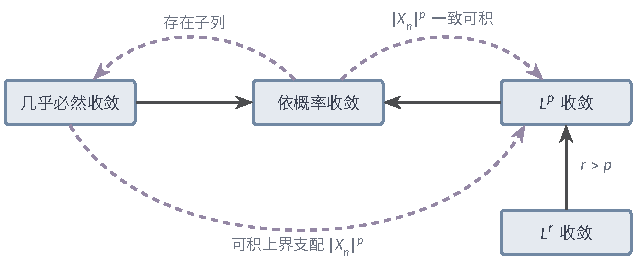
\includegraphics[width=108mm]{figures/07-probability/03-probability-limits/tikz/rvconv-implications/figure.pdf}
 \caption{同一概率空间上收敛方式之间的关系，$1\leq p<r<\infty$。深灰实线箭头总是成立；紫色虚线箭头在所标条件下成立：依概率收敛的列存在几乎必然收敛的子列，依概率收敛加上$\{\lvert X_n\rvert^{p}\}$一致可积推出$L^{p}$收敛，几乎必然收敛加上$\lvert X_n\rvert^{p}$有共同可积上界推出$L^{p}$收敛。}
 \label{fig:rvconv-implications}
\end{BookInlineFigure}

几乎必然行为由事件的重复来判断。误差最终小于$\varepsilon$，就是超差事件只发生有限次；只需对可数个阈值检查。超差概率可以求和时，Borel–Cantelli引理不需要任何独立性就保证有限次发生；概率不可求和时，只有在独立条件下才能断言无穷多次发生，没有独立性则什么都推不出。依概率收敛的列总有几乎必然收敛的子列，而依概率收敛恰好等价于“每个子列都有几乎必然收敛的进一步子列”。

期望与极限的交换由尾部控制决定。单调递增的非负列不会丢失期望，极限期望可以为无穷。不单调时，Fatou引理只给出单向的不等式，丢失的部分是逃到远处的质量。共同的可积上界阻止质量逃逸，给出支配收敛；它真正控制的是整族变量在大取值处的贡献，把这一点单独拿出来就是一致可积性。共同上界和高于一阶的一致矩界都推出一致可积，一阶矩一致有界则不够。在依概率收敛的前提下，$L^{1}$收敛与一致可积等价。平均绝对误差的消失还要和有符号期望的收敛区分开，对非负变量两者才等价。

下一章研究独立随机变量的部分和与样本平均，检验它们怎样满足本章的这些要求：有限方差给出均方误差的估计和依概率收敛，强大数律则要用到几乎必然收敛的判别工具。本章始终要求各变量定义在同一个概率空间上，误差$X_n-X$才有意义；只比较各自的分布、不要求共同实现的收敛由第~\ref{chap:weak-convergence-of-distributions}章研究。
